% !TEX root = ../DP_Vik_Tomas_2013.tex
\chapter{Implementace}
Pro lepší přestavu bude nejdříve zběžně popsán způsob, jakým se všeobecně sestavuje aplikace ve frameworku Ruby on Rails. Následně se bude kapitola věnovat detailněji implementaci napojení aplikace na srovnávač Heureka.cz, implementací získávání aktuálních cen a jejich zpracování do grafu a na konci kapitoly bude ukázka implementovaných obrazovek aplikace.

\section{Standardní rozvržení aplikace v Ruby on Rails}
Jak již bylo řečno v kapitole \ref{sec:ror}, aplikace upřednostňuje konvenci před konfiguraci, což na jednu stranu znamená minimum konfigurace aplikace, na druhou stranu to znamená že má vývojář přesně dané postupy jak v implementaci něčeho dosáhnout. Framework je postaven na návrhovém vzoru MVC a to také implementaci rozděluje na tři významné části.

\subsection{Model}
Model reprezentuje informace v aplikaci a pravidla jak s nimi zacházet. Což se dá interpretovat také jako mechanismus zapisování a čtení databáze a pravidla tohoto zápisu/čtení. Model je v Rails řešen pomocí knihovny Active Record. Ta poskytuje nad každým objektem modelu velkou škálu funkcí ketré manipulují přímo s databází. Každá modelová třída musí dědit od |ActiveRecord::Base|. Na schématu \ref{fig:model-diagram} jsou vidět všechny modelové třídy ve výsledné aplikaci. Každý model v Rails má v příslušené tabulce v databázi ještě dva sloupce |create_at| a |updated_at| jejichž hodnoty se automaticky nastavují při vytvoření/upravení záznamu.

\begin{figure}[htb]
\begin{center}
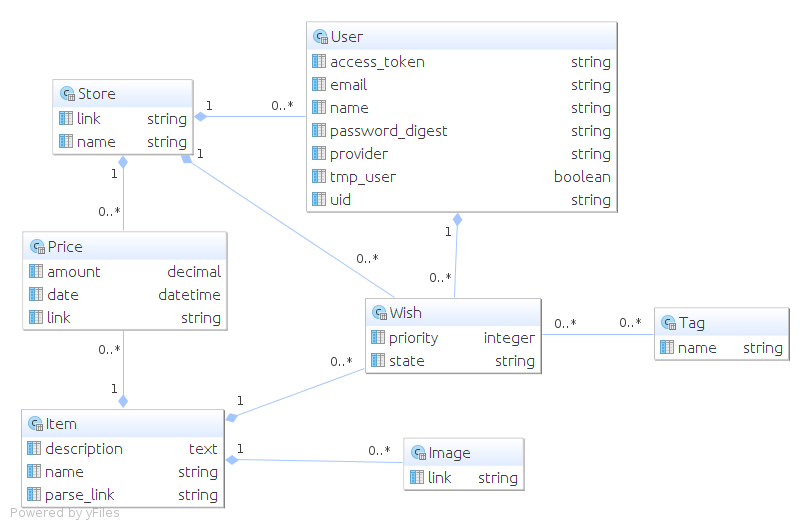
\includegraphics[width=120mm]{./pictures/model-diagram.png}
\caption{Digram tříd v modelu aplikace}
\label{fig:model-diagram}
\end{center}
\end{figure}

\subsection{Controller}
Controller je v Rails třída, která dědí od třídy |ActionController::Base|. Tato třída má na starosti zpracování HTTP dotazů. Pokud přijde dotaz, framework se pokusí v routes souboru\footnote{Konfigurační soubor, ve kterém jsou nastaveny pro každou validní URL odpovídající controllery a jejich metody.} najít vhodný controller a jeho metodu kterou poté zavolá. Controller má mimo jiné přístup k parametrům se kterými byl proveden HTTP dotaz a k session proměnné.

Dále je v Rails aplikacích standardem, že existuje controller, který se nazývá |ApplicationController| a od něj dědí všechny ostatní controllery. Tak je tomu i ve výsledné aplikaci.

V následující ukázce je kus kódu největšího controlleru výsledné aplikace |WishesController|. Konkrétně metoda, která se volá po odeslání formuláře na přidání přání.

\lstset{language = ruby, style=custom}
\begin{lstlisting}
class WishesController < ApplicationController

#....... kod vynechan

  # POST /wishes
  # POST /wishes.json
  def create
    #ziskame prani pro id z parametru
    @wish = Wish.new(params[:wish])
    #z retezce ziskame stitky
    tags = Tag.parse_tags(params[:tags])
    @wish.tags = tags
    @wish.user = current_user
    #inicializujeme prioritu prani
    @wish.initialize_priority(params[:user_priority].to_d)
    respond_to do |format|
      format.html { redirect_to wishes_path, notice: :success }
      format.json { render json: @wish, status: :created, location: @wish }
    end
  end

#....... kod vynechan

end
\end{lstlisting}

\subsection{View}
View reprezentuje uživatelské rozhranní aplikace